\documentclass[titlepage]{article}
\usepackage{minted}
\usepackage[margin=0.5in]{geometry}
\usepackage{graphicx}

\title{Internet Technologies Lab Report\\Assignment 2}
\author{Md Sahil\\BCSE IV\\Roll-001710501029}
\date{}

\begin{document}
    {\maketitle}

    \section{Problem Statement}
    Write a multi-client chat application consisting of both client and server programs.
    In this chat application simultaneously several clients can communicate with each other.
    For this you need a single server program that clients connect to.
    The client programs send the chat text or image (input) to the server and then the server
    distributes that message (text or image) to all the other clients.
    Each client then displays the message sent to it by the server.
    The server should be able to handle several clients concurrently.
    It should work fine as clients come and go.
    

    Develop the application using a framework based on Node.JS.\@
    How are messages handled concurrently? Which web application framework(s) did you follow?  
    Prepare a detailed report of the experiments you have done, and your observations on the protocol layers thus created.  

    \section{Development stack used}
    \begin{itemize}
        \item Server:
            \begin{itemize}
                \item Node js
                \item Express js
                \item Socket.io
            \end{itemize}
        \item Client:
            \begin{itemize}
                \item React js
                \item Socket.io
            \end{itemize}
    \end{itemize}

    \section{Usage and Features}
    \textbf{DingDing} is an online real time chat application with support for images and text.
    Users can create accounts on the platform. User Id and password are stored for each user in the server.
    Users can connect with other users through their respective user Ids. Multicast groups can also be formed.
    A group consists of more than one users. There is also a broadcast group. Every user in the platform by default
    is present in that group and thus sending messages there reaches everyone in the platfrom.
    \\~
    \\~
    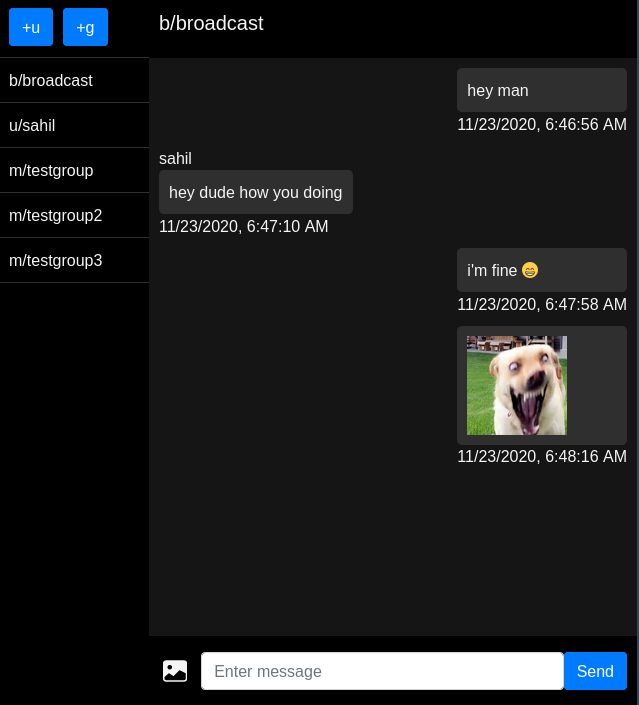
\includegraphics[width=10cm]{./ss.png}

    \section{Design \& Implementation}
    
    \subsection{Directory structure}
    \begin{minted}{bash}
.
|-- LICENSE
|-- README.md
|-- client
|   |-- build
|   |-- package-lock.json
|   |-- package.json
|   |-- public
|   |   |-- index.html
|   |   |-- manifest.json
|   |   `-- robots.txt
|   `-- src
|       |-- App.css
|       |-- App.js
|       |-- components
|       |   |-- ChatScreen.js
|       |   |-- ChatWindow.js
|       |   |-- LoginScreen.js
|       |   |-- MessageBox.js
|       |   `-- SidePanel.js
|       `-- index.js
|-- docs
|   `-- res
|       `-- ss.png
|-- package-lock.json
|-- package.json
`-- server
    |-- register.js
    |-- register_data.json
    `-- server.js
    \end{minted}

    \subsection{Framework}
    The server build on nodejs has two parts i.e. a Rest API part and a websocket part.
    Client data like user\_id, password, list of connections, groups are stored in the server.

    \subsubsection{User data stored in server}
    Example user data stored in server:
    \begin{minted}{json}
      "sahil": {
          "password": "test",
          "connections": {
              "broadcast": {
                  "type": "b"
              },
              "bikram": {
                  "type": "u"
              },
              "irin": {
                  "type": "u"
              "Jucse": {
                  "type": "m",
                  "users": [
                      "bikram",
                      "irin",
                      "sahil"
                  ]
              },
              "memes": {
                  "type": "m",
                  "users": [
                      "bikram",
                      "sahil"
                  ]
              }
          }
      }
    \end{minted}
    
    Example group data stored in the server
    \begin{minted}{json}
          "Jucse": {
              "type": "m",
              "users": [
                  "bikram",
                  "irin",
                  "sahil"
              ]
          }
    \end{minted}

    Here \emph{type} \emph{u} stands for unicast, \emph{m} stands for multicast
    and \emph{b} stands for broadcast.
    The broadcast group is present by default for each user.

    \subsubsection{The Rest API} 
    The Rest API part of the server handles the following tasks:
    \begin{itemize}
        \item user signup
        \item user login and fetch user data
        \item add connection
        \item create new group
    \end{itemize}

    \subsubsection{The Web Socket}
    The web socket part is used for the transfer of realtime messages.
    Messages are structured as json objects\\
    Message structure:
    \begin{minted}{text}
        {
            "contentType" : "..." // text or other media
            "type: : "...", // unicast, multicast, broadcast
            "body" : "...",
            "timestamp" : "...",
            "receiver" : "...",   // uid or gid or broadcast message
            "sender" : "...", // Id of user who wrote the message
        }
    \end{minted}

    When a message is sent from the client side, the server reads the message object, checks the sender and receiver and
    forwards the message to the correct user or group memebers accordingly.


    In order to send image data images are converted into \emph{base64} strings.
    The \textit{contentType} field of the message json is set to \emph{img} and
    the \emph{base64 string} is set as the \textit{body} field of the message json.

    \section{Comments}
    Currently the app is hosted on a heroku dyno.
    There are a number of issues with the app, like, it doesnot work in mobile browsers.
    Also the socket disconnects if kept idle for long periods of time.
    There are also features left to be implemented in the future like message read receipts.

\end{document}
